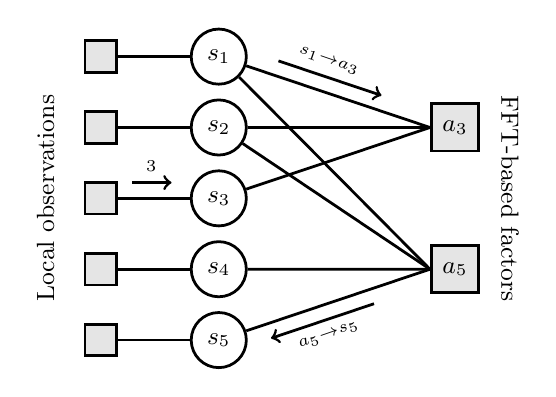
\begin{tikzpicture}
  [
  font=\small, line width=1pt, draw=black,
  check/.style={rectangle, minimum height=6mm, minimum width=6mm, draw=black, fill=gray!20},
  trivialcheck/.style={rectangle, minimum height=4mm, minimum width=4mm, draw=black, fill=gray!20},
  section/.style={circle, minimum size=7mm, draw=black}
  ]

\foreach \m in {1,2,3,4,5} {
  \node[section] (s\m) at (0,2.7-0.9*\m) {$s_{\m}$};
}

\foreach \t in {1,2,3,4,5} {
  \node[trivialcheck] (t\t) at (-1.5,2.7-0.9*\t) {}
    edge (s\t);
}

\node[check] (a3) at (3,0.9) {$a_3$};
\node[check] (a5) at (3,-0.9) {$a_5$};

\node[rotate=90] (variable) at (-2.2,0) {Local observations};
\node[rotate=-90] (check) at (3.7,0) {FFT-based factors};

\draw (s1) -- (a3.west);
\draw (s2) -- (a3.west);
\draw (s3) -- (a3.west);
\draw (s1) -- (a5.west);
\draw (s2) -- (a5.west);
\draw (s4) -- (a5.west);
\draw (s5) -- (a5.west);

\draw[shorten <=0.8cm,shorten >=0.65cm,->] (s1)++(0,0.2cm) -- node[above,rotate=-19] {$\muv_{s_1 \to a_3}$} ([yshift=0.2cm]a3.west);
\draw[shorten <=0.7cm,shorten >=0.75cm,<-] (s5)++(0,-0.2cm) -- node[below,rotate=19] {$\muv_{a_5 \to s_5}$} ([yshift=-0.2cm]a5.west);
\draw[shorten <=0.4cm,shorten >=0.4cm,->] (t3)++(0,0.2cm) -- node[above] {$\lambdav_3$} (-0.2,0.2cm);

\end{tikzpicture}
